\documentclass[12pt]{article}
\usepackage{amsfonts,amssymb,amsmath}
\usepackage{graphicx}
\usepackage{listings}
\usepackage{color} %red, green, blue, yellow, cyan, magenta, black, white
\definecolor{mygreen}{RGB}{28,172,0} % color values Red, Green, Blue
\definecolor{mylilas}{RGB}{170,55,241}
%\documentstyle[12pt,amsfonts]{article}
%\documentstyle{article}

\setlength{\topmargin}{-.5in}
\setlength{\oddsidemargin}{0 in}
\setlength{\evensidemargin}{0 in}
\setlength{\textwidth}{6.5truein}
\setlength{\textheight}{8.5truein}
%\input ../basicmath/basicmathmac.tex
%
%\input ../adgeomcs/lamacb.tex
\input ../Cis515_HW3/mac-new.tex
\input ../Cis515_HW3/mathmac.tex

\def\fseq#1#2{(#1_{#2})_{#2\geq 1}}
\def\fsseq#1#2#3{(#1_{#3(#2)})_{#2\geq 1}}
\def\qleq{\sqsubseteq}

%
\begin{document}


\lstset{language=Matlab,%
    %basicstyle=\color{red},
    breaklines=true,%
    morekeywords={matlab2tikz},
    keywordstyle=\color{blue},%
    morekeywords=[2]{1}, keywordstyle=[2]{\color{black}},
    identifierstyle=\color{black},%
    stringstyle=\color{mylilas},
    commentstyle=\color{mygreen},%
    showstringspaces=false,%without this there will be a symbol in the places where there is a space
    numbers=left,%
    numberstyle={\tiny \color{black}},% size of the numbers
    numbersep=9pt, % this defines how far the numbers are from the text
    emph=[1]{for,end,break},emphstyle=[1]\color{red}, %some words to emphasise
    %emph=[2]{word1,word2}, emphstyle=[2]{style},    
}


\begin{center}
\fbox{{\Large\bf Fall 2016 \hspace*{0.4cm} CIS 515}}\\
\vspace{1cm}
{\Large\bf Fundamentals of Linear Algebra and Optimization\\
Jean Gallier \\
\vspace{0.5cm}
Homework 3}\\[10pt]
October 25, 2016\\
Francine Leech, Reffat Manzur, Chen Xiang \\
\end{center}


\vspace {0.25cm}\noindent
{\bf Problem B1 (20 pts).} \\
Let us prove this first for two subspaces. $E = U_1 \oplus U_2$ if and only if $$ (1)\ E = U_1  + U_2$$ and $$(2)\ U_1 \cap U_2 = {0}$$. 

For $(1)$, every vector $e \in E$ can be uniquely written as $e = u_{11} + u_{21}$ with $u_{11} \in U_1$ and $u_{21} \in U_2$. \\

For $(2)$, let $e \in U_1 \cap U_2$. Since $e \in U_1$ and $e \in U_2$, then we can write, \\

$(1)\ e = e + 0$ where $e \in U_1$ and $0 \in U_2$ and  \\

$(2)\ e = 0 + 0$ where $0 \in U_1$ and $e \in U_2$.  \\ 

But $e = u_{11} + u_{21}$ is unique, so $e=0$. Since $E = U_1 + U_P$, we will check uniqueness. Suppose $e = u_{11} + u_{21}$ and $e = u_{12} + u_{22}$ where $u_{11} , u_{12}  \in U_1$ and $u_{21} , u_{22}  \in U_2$. Then $u_{11} + u_{21} = u_{12} + u{22}$, so $u_{11} - u_{12} = u_{22} - u_{21}$.  Let $x$ be a vector such that $x = u_{11} - u_{12} = u_{22} - u_{21}$. Then $x \in U_1$ and $x \in U_2$, and $u_{11} = u_{12}$ and $u_{22} = u_{21}$, so $x \in U_1 \cap U_2 = (0)$. \\

Now by induction we can extend our logic for any number of $p\geq 2$  subspaces of some vector space $E$. 



\vspace {0.25cm}\noindent
{\bf Problem B2 (50 pts).}

\medskip
(1)\\

By definition an involution is a function $f$ that is its own inverse. \\

$f: E \rightarrow E$ is in an involution when $\forall x \in E: f(f(x)) = x$. Since $f^{-1} = f$, we just have to check that $f(f(x)) =x$ for all x in the domain of f. \\

Let us find the inverse of $f(x) = b -x$ where b is any real number. Let,  
$$f(x) = a -x$$
$$y=a-x$$
$$f^{-1} = a - y $$
$$ x = a-y$$
$$y= a-x$$
so $f(x) = f^{-1}(x)$. So it's an inverse of itself. \\

\medskip
(2)\\

Let $u_1 = \frac{u + f(u)}{2}$ and $u_{-1} = \frac{u-f(u)}{2}$. \\

Next, we can find that we have something in both the spaces. 
$f(u_1) = f(\frac{u+f(u)}{2}) = \frac{f(u) + f(f(u))}{2} = \frac{f(u) + u}{2} = u_1$ \\
$f(u_{-1}) = f(\frac{u-f(u)}{2}) = \frac{f(u)-f(f(u))}{2} = \frac{f(u) - u}{2} = u_{-1}$. \\

Next we need to look at uniqueness. Let $v_1 \in E_1 and \in E_{-1}$. \\
$f(v_1) = v_1$ \\
$f(v_1) = -v_1$ \\
$v_1 = -v_1$ can only have this if $v_1 = -v_1 = 0$. 



\medskip
(3)
Let the basis of $E$ be $(\xi_i), i = 1, 2, \cdots, n$, where $\xi_i = 
\begin{pmatrix}
0 \\
0 \\
\vdots \\
1_i \\
0 \\
\vdots \\
0 \\
\end{pmatrix}
$.Define \\
$
f(\xi_i) = \left \{
				\begin{array}{ll}
				\xi_i \; i = 1,2,\cdots,k \\
				-\xi_i \; i = k+1, k+2, \cdots, n				
				\end{array}
			\right.
$. Then $\forall u \in E$, we can write as $u = \sum_i \lambda_i \xi_i$ and $f(u) = 
\begin{pmatrix}
\xi_1 \\
\xi_2 \\
\vdots \\
\xi_k \\
-\xi_{k+1} \\
-\xi_{k+2} \\
\vdots \\
-\xi_n
\end{pmatrix} 
= I_{k , n - k} \cdot u
$. 
And $
(f \circ f)(u) = I_{k , n - k}I_{k , n - k}  I_{k , n - k}  u = I u = u
$. Thus $f$ is an involution.\\
Geometric interpretation of the action of $f$ is that $f(u)$ is the reflection of $u$ across some axises. When $k = n - 1$, we can easily find that $f(u)$ differs from $u$ only in the last entry $f(u)_i = -u_i$, so it is the reflection across the $n^{th}$ axis.

\vspace {0.5cm}\noindent
{\bf Problem B3 (50 pts).}


\medskip
(1)\\
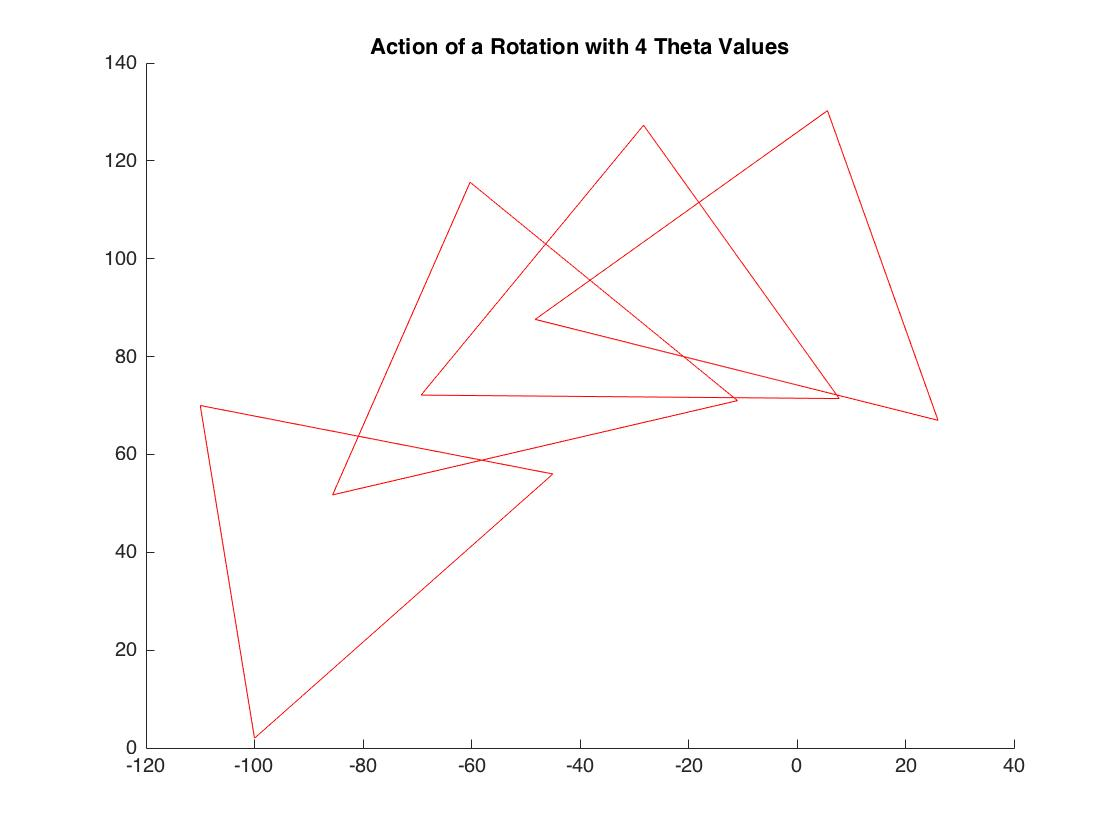
\includegraphics[scale=.25]{RotationPlot}

\medskip
(2)
\[
\begin{pmatrix}
\cos\theta & -\sin\theta \\
\sin\theta & \cos\theta
\end{pmatrix}
\cdot
\begin{pmatrix}
\cos(-\theta) & -\sin(-\theta) \\
\sin(-\theta) & \cos(-\theta)
\end{pmatrix}
\]

\[
=
\begin{pmatrix}
\cos(1) & -\sin(1) \\
\sin(1) & \cos(1)
\end{pmatrix}
\cdot
\begin{pmatrix}
\cos(-1) & -\sin(-1) \\
\sin(-1) & \cos(-1)
\end{pmatrix}
\]
\[
=
\begin{pmatrix}
(\cos\theta \cdot \cos(-\theta)) \cdot (-\sin\theta \sin(-\theta)) & -\cos(\theta)0 \\
\sin(\theta)cos(-\theta)+cos\theta \sin(-\theta) & 1\cos(1)
\end{pmatrix}
=
\begin{pmatrix}
1 & 0 \\
0 & 1
\end{pmatrix}
\]

\medskip
(3) Because $
\cos(\alpha + \beta) = \cos \alpha \cos \beta  - \sin \alpha \sin \beta,
\sin(\alpha + \beta) = \sin \alpha \cos \beta + \cos \alpha \sin \beta
$, we have 
\begin{align*}
R_{\alpha} \circ R_{\beta} &= 
\begin{pmatrix}
\cos\alpha & -\sin\alpha \\
\sin\alpha & \cos\alpha
\end{pmatrix} 
\cdot
\begin{pmatrix}
\cos\beta & -\sin\beta \\
\sin\beta & \cos\beta
\end{pmatrix} \\
&= R_{\beta} \circ R_{\alpha} 
= R_{\alpha + \beta}
\end{align*}
We can get 
\begin{align*}
&1. (R_{\alpha} \circ R_{\beta}) \circ R_{\gamma} = R_{\alpha + \beta + \gamma} = R_{\alpha} \circ (R_{\beta} \circ R_{\gamma}) \\
&2. R_{\alpha} \circ I = I \circ R_{\alpha} = R_{\alpha} \\
&3. R_{\alpha} \circ R_{-\alpha} = I \\
&4. R_{\alpha} \circ R_{\beta} = R_{\alpha + \beta} = R_{\beta} \circ R_{\alpha}
\end{align*}
So rotations in the plane form a commutative group.

\vspace {0.5cm}\noindent
{\bf Problem B4 (110 pts).}

\medskip
(1)We can write 
$\begin{pmatrix}
c_1\\
c_2
\end{pmatrix} = R_{\theta,(a_1,a_2)} \begin{pmatrix}
c_1\\
c_2
\end{pmatrix}$ as:

\vspace{0.25cm}
 \[\begin{pmatrix}
c_1\\
c_2
\end{pmatrix}= \begin{pmatrix}
  cos\theta & -sin\theta\\
  sin\theta & cos\theta
  \end{pmatrix}\begin{pmatrix}
c_1\\
c_2
\end{pmatrix} +\begin{pmatrix}
a_1\\
a_2
\end{pmatrix}\]
  
Then,
\begin{equation}
c_1 = cos\theta c_1 - sin\theta c_2 + a_1 \end{equation}
\begin{equation} c_2 = sin\theta c_1 + cos\theta c_2 + a_2 \end{equation}

Using the result for $(c_1,c_2)$ as given in the problem and by substituting, we will check if the equations are true for when $\theta\ne k2\pi$.\\

For $c_1$, we are given that
  
$$c_1=\frac{1}{2sin\frac{\theta}{2}} (cos(\frac{\pi - \theta}{2})a_1)- sin(\frac{\pi- \theta}{2})a_2)$$


 $\frac{1}{2}\frac{cos(\frac{\pi - \theta}{2})}{sin\frac{\theta}{2}}$ simplifies to $\frac{1}{2}$.

 $\frac{-1}{2}\frac{sin(\frac{\pi - \theta}{2})}{sin\frac{\theta}{2}}$ simplifies to $ \frac{1}{2}cot \frac{\theta}{2}$.

so: $$c_1 = \frac{1}{2} (a_1 - cot \frac{\theta}{2}a_2)$$

Similarly, for $c_2$,  it becomes
$$c_2= \frac{1}{2}cot\frac {\theta}{2}a_1 + \frac{1}{2}a_2$$

Now by substitution into equation (1), we get :

$$\frac{1}{2} (a_1 - cot \frac{\theta}{2}a_2)$$

$$=cos\theta(\frac{1}{2} (a_1 - cot \frac{\theta}{2}a_2)) - sin\theta(\frac{1}{2}cot\frac {\theta}{2}a_1 + \frac{1}{2}a_2) + a_1$$

$$=(\frac{cos\theta}{2} - \frac{sin\theta}{2}cot\frac{\theta}{2} +1)a_1 - \frac{1}{2}(cos\theta cot\frac{\theta}{2} + sin\theta)a_2$$


Then, $cos\theta - sin\theta cot \frac{\theta}{2} = -1$ and $cos\theta cot \frac{\theta}{2} + sin\theta = cot \frac{\theta}{2}$

so equation (1) on the right hand side simplifies to  $c_1 = \frac{1}{2} (a_1 - cot \frac{\theta}{2}a_2)$ and matches the left hand side of equation (1).

For equation (2), we get:

$$\frac{1}{2}cot\frac {\theta}{2}a_1 + \frac{1}{2}a_2$$

$$=sin\theta\frac{1}{2} (a_1 - cot \frac{\theta}{2}a_2)+ cos\theta(\frac{1}{2}cot\frac {\theta}{2}a_1 + \frac{1}{2}a_2) + a_2$$

$$=(\frac{sin\theta}{2} + (\frac{1}{2} cos\theta cot\frac{\theta}{2}))a_1 +((\frac{-1}{2}sin\theta cot\frac{\theta}{2} + \frac{cos\theta}{2} +1)a_2$$

Thus, the right hand side of equation (2) simplifies and $c_2= \frac{1}{2}cot\frac {\theta}{2}a_1 + \frac{1}{2}a_2$.



It is then clear that the unique fixed point is $(c_1,c_2)$ where $\theta\ne k2\pi$ because $cot\frac{\theta}{2}$ is undefined for where $\theta$ is a multiple of $2\pi$.


\medskip
\vspace{0.25 cm}
(2) 

\[\begin{pmatrix} y'_1 + c_1\\y'_2 + c_2 \end{pmatrix} = \begin{pmatrix} cos\theta & -sin\theta \\ 
sin\theta & cos\theta \end{pmatrix} \begin{pmatrix} x'_1 + c_1\\x'_2 + c_2 \end{pmatrix} + \begin{pmatrix} a_1 \\ a_2 \end{pmatrix}\]

\[y'_1 + \frac{1}{2}(a_1 - cot\frac{\theta}{2} a_2) =  cos\theta x'_1 + cos\theta (\frac{1}{2}(a_1 - cot \frac{\theta}{2} a_2)) - sin\theta x'_2 - sin\theta (\frac{1}{2} (cot \frac{\theta}{2}a_1 + a_2)) + a_1 \]

$$ = cos\theta x'_1  - sin\theta x'_2 + (\frac {cos\theta}{2} + 1 - (\frac{sin\theta cot \frac{\theta}{2}}{2} ))a_1 - \frac{1}{2}(cos\theta cot \frac{\theta}{2} + sin\theta) a_2$$

Using $cos\theta - sin\theta cot \frac{\theta}{2} = -1$ and $cos\theta cot \frac{\theta}{2} + sin\theta = cot \frac{\theta}{2}$, the $\frac{1}{2} (a_1 - cot \frac{\theta}{2}a_2)$ cancel out from both sides of the equation and then $$y'_1 = cos\theta x'_1 - sin\theta x'_2$$.
$$y'_2 + c_2 = sin\theta (x'_1+ c_1) + cos\theta (x'_2 +c_2) + a_2$$

By substituting $\frac{1}{2} \left( cot \frac{\theta}{2} a_1+a_2 \right)$ for $c_2$ and $\frac{1}{2} \left( -cot \frac{\theta}{2} a_2+a_1 \right)$ for $c_1$, we get\\ 

 $$y'_2 = sin\theta x'_1 + cos\theta x'_2$$
 
 Thus, the original affine map becomes 
 
 $$ \begin{pmatrix}y'_1 \\y'_2\end{pmatrix}= R_\theta \begin{pmatrix}x'_1 \\x'_2\end{pmatrix}$$

\medskip
(3)
Use {\tt Matlab} to show the action of  the affine map
$R_{\theta, (a_1,a_2)}$ on a simple figure such as
a triangle or a rectangle,
for $\theta = \pi/3$ and various values of $(a_1, a_2)$.
Display the center $(c_1, c_2)$ of the rotation.

\medskip
What kind of transformations correspond to
$\theta= k 2\pi$, with $k \in \integs$?
The four centers of rotation in the figure are represented by *.\\
When $\theta = k2\pi$, we have $cos\theta=1$ and $sin\theta=0$, 
so $y_1 = x_1 + a_1$ and $y_2=x_2 + a_2$ and this indicates the transformation is a translation.

\medskip
(4) \\

$R_{\theta, (a_1,a_2)}$ \\
\[
\begin{pmatrix}
y_1 \\
y_2 \\
1
\end{pmatrix}
=
\begin{pmatrix}
\cos\theta & -\sin\theta & a_1 \\
\sin\theta & \cos\theta & a_2 \\
0 & 0 & 1 \\
\end{pmatrix}
\begin{pmatrix}
x_1 \\
x_2 \\
1 \\
\end{pmatrix}
\]

$R_{-\theta, (b_1,b_2)}$ \\
\[
\begin{pmatrix}
y_1 \\
y_2 \\
1
\end{pmatrix}
=
\begin{pmatrix}
\cos(-\theta) & -\sin(-\theta) & b_1 \\
\sin(-\theta) & \cos(-\theta) & b_2 \\
0 & 0 & 1 \\
\end{pmatrix}
\begin{pmatrix}
x_1 \\
x_2 \\
1 \\
\end{pmatrix}
=
\begin{pmatrix}
\cos(\theta) & \sin(\theta) & b_1 \\
-\sin(\theta) & \cos(\theta) & b_2 \\
0 & 0 & 1 \\
\end{pmatrix}
\begin{pmatrix}
x_1 \\
x_2 \\
1 \\
\end{pmatrix}
\] \\

\[
R_{\theta, (a_1,a_2)} \cdot R_{-\theta, (b_1,b_2)} =
\begin{pmatrix}
\cos\theta & -\sin\theta & a_1 \\
\sin\theta & \cos\theta & a_2 \\
0 & 0 & 1 \\
\end{pmatrix}
\begin{pmatrix}
\cos(\theta) & \sin(\theta) & b_1 \\
-\sin(\theta) & \cos(\theta) & b_2 \\
0 & 0 & 1 \\
\end{pmatrix}
\]
\[
=
\begin{pmatrix}
\cos^2\theta + \sin^2\theta & cos\theta \sin\theta - cos\theta \sin\theta & \cos\theta b_1 - \sin \theta b_2 + a_1 \\
cos\theta \sin\theta - cos\theta \sin\theta & \sin^2\theta + \cos^2\theta  & \sin\theta b_1 + \cos\theta b_2 + a_2\\
0 & 0 & 1 \\
\end{pmatrix}
\]
\[
=
\begin{pmatrix}
1 & 0 & 0 \\
0 & 1  & 0 \\
0 & 0 & 1 \\
\end{pmatrix}
\]

So $\cos\theta b_1 - \sin \theta b_2 + a_1 = 0$ and $\sin\theta b_1 + \cos\theta b_2 + a_2 = 0$. \\

Solve for $b_1$, \\
$b_1 = \frac{- a_1 +  \sin \theta b_2}{\cos\theta}$ \\
$b_1 = \frac{- a_1}{\cos\theta} + \frac{\sin \theta b_2}{\cos\theta}$ \\
$b_1 = -\sec\theta a_1 + \tan\theta b_2$ \\

Solve for $b_2$, \\
$b_2 = \frac{- a_2 +  \sin \theta b_1}{\cos\theta}$  \\
$b_2 = \frac{- a_2}{\cos\theta} - \frac{\sin \theta b_1}{\cos\theta}$ \\
$b_2 = \sec\theta a_2 - \tan\theta b_1$ \\

Now plug in $b_2$ into $b_1$.

$b_1 = -\sec\theta a_1 + \tan\theta (\sec\theta a_2 - \tan\theta b_1)$ \\
$b_1 = \sec\theta a_1 - \tan\theta \sec\theta a_2 - \tan^2\theta b_1$ \\
$(1-tan^2\theta)b_1 = \sec\theta a_1 - \tan\theta \sec\theta a_2 $ \\
$b_1 = \frac{-\tan \theta}{\sec \theta}a_2 - \cos \theta a_1$ \\
$b_1 = - \sin \theta a_2 - \cos \theta a_1$ 

Now plug $b_1$ into $b_2$ we get, 
$b_2 = \sin \theta a_1 - \cos \theta a_1$. \\

The final answer for $b_1$ and $b_2$ in terms of $\theta$, $a_1$, and $a_2$ is, 
$$b_1 = -\sin \theta a_2 - \cos \theta a_1$$
$$b_2 = \sin \theta a_1 - \cos \theta a_1$$

\medskip
(5)

<<<<<<< Updated upstream
$R_{\beta,(b_1,b_2)}:$

$$\begin{pmatrix}
y_1\\y_2\\1
\end{pmatrix}=\begin{pmatrix}
cos\beta & -sin\beta & b_1\\ sin\beta & cos\beta & b_2 \\ 0&0&1
\end{pmatrix}\begin{pmatrix}
x_1\\x_2\\1
\end{pmatrix}$$

$R_{\alpha,(a_1,a_2)}:$

$$\begin{pmatrix}
y_1\\y_2\\1
\end{pmatrix}=\begin{pmatrix}
cos\alpha & -sin \alpha & a_1\\ sin\alpha & cos\alpha & a_2 \\ 0&0&1
\end{pmatrix}\begin{pmatrix}
x_1\\x_2\\1
\end{pmatrix}$$

$$R_{\beta,(b_1,b_2)}\circ R_{\alpha,(a_1,a_2)}\rightarrow$$
$$
\begin{pmatrix}
cos\beta & -sin\beta & b_1\\ sin\beta & cos\beta & b_2 \\ 0&0&1
\end{pmatrix}\begin{pmatrix}
cos\alpha & -sin \alpha & a_1\\ sin\alpha & cos\alpha & a_2 \\ 0&0&1
\end{pmatrix}$$
$$= \begin{pmatrix}
cos\beta cos\alpha - sin\beta sin\alpha & -cos\beta sin\alpha - sin\beta cos\alpha & cos\beta a_1 - sin\beta a_2 + b_1\\
sin\beta cos\alpha + cos\beta sin\alpha & -sin\beta sin\alpha + cos\beta cos\alpha & sin\beta a_1 + cos\beta a_2 + b_2 \\0&0&1

\end{pmatrix}$$

Using the trig identities from part 4, we get:
$$\begin{pmatrix}
cos(\alpha + \beta)& -sin(\alpha + \beta) & t_1\\
sin(\alpha + \beta) & cos(\alpha + \beta) & t_2 \\
0&0&1
\end{pmatrix}$$

Indeed, this matrix represents $R_{\alpha + \beta,(t_1,t_2)}$ where $t_1 = cos\beta a_1 - sin \beta a_2 + b_1$ and $t_2 = sin\beta a_1 + cos\beta a_2 + b_2$.

Furthermore, 
$$R_{\beta,(b_1,b_2)} \circ R_{\alpha} \rightarrow$$
$$
\begin{pmatrix}
cos\beta & -sin\beta & b_1\\ sin\beta & cos\beta & b_2 \\ 0&0&1
\end{pmatrix}\begin{pmatrix}
cos\alpha & -sin\alpha & 0\\ sin\alpha & cos\alpha & 0 \\ 0&0&1
\end{pmatrix}$$
$$=\begin{pmatrix}
cos(\alpha + \beta)& -sin(\alpha + \beta) & b_1\\
sin(\alpha + \beta) & cos(\alpha + \beta) & b_2 \\
0&0&1
\end{pmatrix}$$

However, $R_\alpha \circ R_{\beta,(b_1,b_2)}\rightarrow$
$$\begin{pmatrix}
cos\alpha & -sin\alpha & 0\\ sin\alpha & cos\alpha & 0 \\ 0&0&1
\end{pmatrix}\begin{pmatrix}
cos\beta & -sin\beta & b_1\\ sin\beta & cos\beta & b_2 \\ 0&0&1
\end{pmatrix}$$
$$=
\begin{pmatrix}
cos(\alpha + \beta)& -sin(\alpha + \beta) & cos\alpha b_1 - sin\alpha b_2\\
sin(\alpha + \beta) & cos(\alpha + \beta) &sin\alpha b_1 + cos\alpha b_2 \\
0&0&1
\end{pmatrix}$$
 so generally, $$R_{\beta,(b_1,b_2)} \circ R_{\alpha} \ne R_\alpha \circ R_{\beta,(b_1,b_2)}$$ 
=======
Use (4)-(5) to show that the affine maps of the plane defined in this
problem form a nonabelian group denoted $\mathbf{SE}(2)$.

\medskip
Prove that  $R_{\beta, (b_1,b_2)} \circ R_{\alpha, (a_1,a_2)}$ is
not a translation (possibly the identity)  iff
$\alpha + \beta \not= k 2\pi$, for all  $k\in \integs$.
Find its center of rotation when $(a_1, a_2) = (0, 0)$.  

\medskip
If $\alpha + \beta = k 2\pi$, then  $R_{\beta, (b_1,b_2)} \circ
R_{\alpha, (a_1,a_2)}$
is a pure translation. 
Find the translation vector 
of $R_{\beta, (b_1,b_2)} \circ R_{\alpha, (a_1,a_2)}$.
>>>>>>> Stashed changes
Since we show that $R_{\beta,(b_1,b_2)} \circ R_{\alpha} \ne R_{\alpha} \circ R_{\beta,(b_1,b_2)}$, the commutative property does not hold so the maps form a nonabelian group.\\

When $\alpha + \beta = k2\pi$, $R_{\beta,(b_1,b_2)} \circ R_{\alpha,(a_1,a_2)}$ is a translation since $cos(\alpha + \beta)= 1$ and $sin(\alpha + \beta)=0$ so the map corresponding to $R_{\beta,(b_1,b_2)} \circ R_{\alpha,(a_1,a_2)}$ becomes:
$$\begin{pmatrix} 1 & 0 & t_1\\0&1& t_2\\0&0&1\end{pmatrix}$$ which represents a translation when applied to a vector. In any other case where $\alpha + \beta \ne k2\pi$, the map will not be a translation.\\

When $(a_1,a_2)=(0,0)$, we can substitute into the equation for the center of rotation and find that $(c_1,c_2)= (0,0)$.\\

When $\alpha + \beta = k2\pi$, the translation vector $(t_1,t_2)$ is defined above where $t_1= cos\beta a_1 - sin\beta a_2 + b_1$ and $t_2 = sin\beta a_1 + cos\beta a_2 + b_2$.

\vspace {0.5cm}\noindent
{\bf Problem B5 (80 pts).}

\medskip
(1)
Because $U$ is a subspace of $\reals^n$, then $0 \in U$, we have $a = 
a + 0 \in \s{A}$
\begin{center}
Affine subspace of dimension 0 are points. \\
Affine subspace of dimension 1 are lines. \\
Affine subspace of dimension 2 are planes. \\
\end{center}
Any $a + u \in \s{A}, \; a + v \in \s{A}$, then the affine combination is $\lambda (a + u) + (1 - \lambda) (a + v) = a + \lambda u + (1 - \lambda) v$, because $U$ is subspace of $\reals^n$, $\lambda u + (1 - \lambda) v \in U$, then $a + \lambda u + (1 - \lambda) v \in \s{A} \Rightarrow \lambda (a + u) + (1 - \lambda) (a + v) \in \s{A}$. Affine subspace is closed under affine combinations.

\medskip
(2) At least from (1) we know $a \in \s{A}$, $\s{A}$ is not empty.
For any $b \in \s{A}$, we can find $u$, write as $b = a + u$. Then   $b - a \in U$, $a + U = a + b - a + U = b + U$.

\medskip
(3)
Choose $x - a \in U_a$, $y - a \in U_a$, $\lambda, \mu \in \reals$, then compute $\lambda (x - a) + \mu (y - a) = \frac{1}{\lambda + \mu}(\frac{\lambda}{\lambda + \mu}(x - a) + \frac{\mu}{\lambda + \mu}(y - a)) = \frac{\lambda}{\lambda + \mu} x + \frac{\mu}{\lambda + \mu} y - a$. Because $\s{A}$ is closed under affine combinations, we have $\frac{\lambda}{\lambda + \mu} x + \frac{\mu}{\lambda + \mu} y \in \s{A}$, then $\lambda (x - a) + \mu (y - a) = \frac{\lambda}{\lambda + \mu} x + \frac{\mu}{\lambda + \mu} y - a \in \reals^n$, $U_a$ is a subspace of $\reals^n$.\\
For any $u \in U_a$, we can write as $u = x - a = x + (b - a) - b$. The sum of coefficients of $x, b, a$ is $1 -1 + 1 = 1$, and $\s{A}$ is closed under affine combinations, then $u = x + (b -a)-b \in \s{A} - b \Rightarrow u \in U_b$. $U_a$ does not depend on the choice of $a \in \s{A}$, $U_a = U_b$ for all $a, b\in \s{A}$.
So $U_a = U = \{y - x \in \reals^n \mid x, y \in \s{A}\}$ and
$
\s{A} = a + U, \quad\hbox{for any $a\in \s{A}$}.
$

\medskip
(4)If $\s{A}\cap \s{B} = (x)$, then we can find $x = a + u = b + v$ where $a \in \s{A}, b \in \s{B}$, $u, v \in U$. Write $b = a + u - v$, thus $b \in \s{A} \Rightarrow \s{A} = \s{B}$, which is against $\s{A} \neq \s{B}$. We have $\s{A} \cap \s{B} = \emptyset$ if $\s{A} \neq \s{B}$ and $\s{A}, \s{B}$ are parallel. 

\vspace {0.25cm}\noindent
{\bf Problem B6 (120 pts).} (Affine frames and affine maps) \\
(1) \\

We can write the $\lambda$'s and $u$'s as a unique linear combination such that, 
$$ \lambda_0 u_0 + \ldots + \lambda_n u_n = 0 $$

Since this is true, the only value for $\sum_{i} \lambda_i$ is 0. We can rewrite this unique linear combination by subtracting $u_0$ from each $u_i$ to get $$\lambda_1 (u_1 - u_0) + \ldots + \lambda_n (u_n - u_0) + \sum_{i}^{n} (u_i + u_0) = 0$$ Since $\sum_{i} \lambda_i = 0$, the linear combination of the difference between $(u_i - u_0)$ is also linearly independent. \\

The subset of a linearly independent set of vectors is also a linearly independent set, so $$\lambda_1 (u_1 - u_0) + \ldots + \lambda_m (u_m - u_0) + \sum_{i}^{m} (u_i + u_0) = 0$$ where $m \leq n$ is linearly independent. Since the difference between the subset of vectors are linearly independent, then $\sum_{i} \lambda_i = 0$ must be true. So $u_0$ can be added to $$\lambda_1 (u_1 - u_0) + \ldots + \lambda_m (u_m - u_0) + \sum_{i}^{m} (u_i + u_0) = 0$$ to get the linear combination, 

$$\lambda_0 \hat{u}_0  + \lambda_1 \hat{u}_1  + \ldots + \lambda_m \hat{u}_m  + = 0$$ Since $\sum_{i} \lambda_i = 0$ is still true, then $\hat{u}_0, \ldots, \hat{u}_m$ are linearly independent.   


\medskip
(2) \\
We proved in $6.1$ that the linear combination $$\lambda_0 \hat{u}_0  + \lambda_1 \hat{u}_1  + \ldots + \lambda_m \hat{u}_m  = 0$$ is linearly independent and $\sum_{i} \lambda_i = 0$. \\

We can rewrite the linear combination by subtracting some $u_i$ from each $u$ to get $$\lambda_0 (\hat{u}_0 - \hat{u}_i)  + \lambda_q (\hat{u}_1 - \hat{u}_i)+ \ldots + \lambda_m (\hat{u}_m - \hat{u}_i) = 0$$ The linear combination can be written by factoring out the $u_i$ to get  $$\lambda_0 \hat{u}_0  + \lambda_1 \hat{u}_1 + \ldots + \lambda_m \hat{u}_m  -  \sum_{i} \lambda_i \hat{u}_i= 0$$

The first set of terms of $m-1$ terms in the equations are a subset of the original $m$ terms from where we started. Since a subset of a linearly independent set is linearly independent, then the $m-1$ terms are linearly independent and $\sum_{i}^{m-1} \lambda_i =0$. This leaves the last term in the equation, $\sum_{i} \lambda_i \hat{u}_i$. We know that the $u$'s are unique, so they cannot equal $0$, this means that the $\lambda_i$'s $=0$. So, the
$m$ vectors $u_j - u_i$  for $j \in \{0, \ldots, m\}$ with $j - i \not = 0$
are linearly independent. 

\medskip
Any $m + 1$ vectors  $(u_0, u_1, \ldots, u_{m })$ such that
the  $m + 1$ vectors
$(\widehat{u}_0, \ldots,  \widehat{u}_m)$ are linearly independent
are said to be {\it affinely independent\/}.

\medskip
From (1) and (2), the vector $(u_0, u_1, \ldots, u_{m })$ 
are affinely independent iff
for any  any choice of $i$, with $0 \leq i \leq m$, the
$m$ vectors $u_j - u_i$  for $j \in \{0, \ldots, m\}$ with $j - i \not = 0$
are linearly independent.
If $m = n$,  we say that $n + 1$ affinely independent 
vectors  $(u_0, u_1, \ldots, u_{n })$ form an {\it affine frame\/} of $\reals^n$. 

\medskip
<<<<<<< Updated upstream
(3) Because $(u_0, u_1, \ldots, u_{n })$ is an affine frame of $\reals^n$, then from above we can get a basis in $\reals^{n+1}$, which is $\widehat{u}_0, \ldots,  \widehat{u}_{n}$. For any $v \in \reals^n$, we denote $\widehat{v} = (v, 1)$, then it can be uniquely written as the combination of $(\widehat{u}_i)$, such that $\widehat{v} = \sum_i \lambda_i \widehat{u}_i$. From the last row of equation, we know there should be $\sum_i \lambda_i = 1$. Along with $v = \sum_i \lambda_i u_i$, we can get the conclusion.\\
\medskip
From $e_i = u_i -  u_0$, for $i = 1, \ldots, n$, substitute $u_i$ with $e_i$, we get $v = \sum_{i=1}^n \lambda_i (e_i + u_0) + \lambda_0 u_0 = \sum_i \lambda_i u_0 + \sum_{i=1}^n \lambda_i e_i = u_0 + \sum_{i=1}^n \lambda_i e_i$.
When $u_i = u_0 + e_i$ for $i = 1, \ldots, n$, denote the vector $\widehat{u_i} = (u_0 + e_i, 1)$. Suppose $\sum_i \lambda_i \widehat{u_i} = 0$, such that
\begin{align*}
\sum_i \lambda_i u_0 + \sum_i \lambda_i e_i &= 0 \\
\sum_i \lambda_i  &= 0 \\ 
\Rightarrow \sum_i \lambda_i e_i &= 0 \\
\Rightarrow \lambda_i &= 0, \; i = 1,2, \cdots, n
\end{align*}
So $\widehat{u}_0, \ldots,  \widehat{u}_{n}$ are linearly independent, thus $(u_0, u_1, \ldots, u_n)$ is an affine frame of $\reals^n$.
From above, for any $v\in \reals^n$, there is $v = u_0 + x_1 e_1 + \dots + x_n e_n$, substitute $e_i$ with $u_i$ get
\[
v = (1 - (x_1 + \cdots + x_x)) u_0 + x_1 u_1 + \cdots + x_n u_n,
\]
=======
(3) if $(u_0, u_1, \ldots, u_{n })$ is an affine frame of $\reals^n$,
then prove that for every vector $v\in \reals^n$,  
there is a unique $(n + 1)$-tuple
$(\lambda_0, \lambda_1, \ldots, \lambda_n)\in \reals^{n + 1}$, with
$\lambda_0 + \lambda_1 + \cdots + \lambda_n = 1$, such that
\[
v = \lambda_0 u_0 + \lambda_1 u_1 + \cdots + \lambda_n u_n.
\]
The scalars $(\lambda_0, \lambda_1, \ldots, \lambda_n)$ are called the
{\it barycentric\/} (or {\it affine\/}) {\it coordinates\/} of $v$
w.r.t. the affine frame   $(u_0, u_1, \ldots, u_{n })$.


(3.1) \\
\medskip
If we write $e_i = u_i -  u_0$, for $i = 1, \ldots, n$, then prove that
we have
\[
v = u_0 + \lambda_1 e_1 + \cdots + \lambda_n e_n,
\]
and since $(e_1, \ldots, e_n)$ is a basis of $\reals^n$ (by (1) \&
(2)), the $n$-tuple $(\lambda_1, \ldots, \lambda_n)$ consists of the 
standard coordinates of $v - u_0$ over the basis $(e_1, \ldots, e_n)$.

(3.2) \\
From above, where $$ \hat{v} = \lambda_0 \hat{u}_0 + \lambda_1 \hat{u}_1 + \ldots + \lambda_n \hat{n}_0$$ are linearly independent. We can rewrite above as, $$\hat{v} = \lambda_1(\hat{u}_1 - \hat{u}_0) + \lambda_2(\hat{u}_2 - \hat{u}_0) + \ldots + \lambda_n(\hat{u}_n - \hat{u}_0) + \sum_{i}^{n} \lambda_i u_0$$
We can replace each $u_i -  u_0$ with $e_i$ such that $e_i = u_i -  u_0$. Now, 
$$\hat{v} = \lambda_1(e_1) + \lambda_2(e_2) + \ldots + \lambda_n(e_n) + \sum_{i}^{n} \lambda_i u_0$$
 

From $6.1$, we know that the subset of a linearly independent set is linearly independent. Thus the first $n-1$ is linearly independent, so the $\sum_{i}^{n-1} \lambda_i = 0$. The last $nth$ term in the equation, $\sum_{i}^{n} \lambda_i u_0$ must equal 0. Since the $u_0$ is unique, the $\lambda_i$'s must equal 0. 
 


\medskip
Conversely, for any vector $u_0\in \reals^n$ and for any basis
$(e_1, \ldots, e_n)$ of $\reals^n$, let
$u_i = u_0 + e_i$ for $i = 1, \ldots, n$. Prove
that $(u_0, u_1, \ldots, u_n)$ is an affine frame of $\reals^n$, 
and for any $v\in \reals^n$, if  
\[
v = u_0 + x_1 e_1 + \dots + x_n e_n,
\]
with $(x_1, \ldots, x_n) \in \reals^n$ (unique), then
\[
v = (1 - (x_1 + \cdots + x_x)) u_0 + x_1 u_1 + \cdots + x_n u_n,
\]
so that $(1 - (x_1 + \cdots + x_x)), x_1, \cdots,  x_n)$,
are the barycentric coordinates of $v$ w.r.t. the affine frame
$(u_0, u_1, \ldots, u_n)$.

(3.3) \\

\medskip
The above shows that there is a one-to-one correspondence between
affine frames $(u_0, \ldots$, $u_n)$ and pairs
$(u_0, (e_1, \ldots, e_n))$, with  $(e_1, \ldots, e_n)$  a basis.
Given  an affine frame  $(u_0, \ldots, u_n)$, we obtain the basis
$(e_1, \ldots, e_n)$ with $e_i = u_i - u_0$, for $i = 1, \ldots, n$;
given the pair $(u_0, (e_1, \ldots$, $e_n))$ where  $(e_1, \ldots, e_n)$
is a basis,  we obtain the affine frame   $(u_0, \ldots, u_n)$, with
$u_i = u_0 + e_i$, for $i = 1, \ldots, n$.
There is also a  one-to-one correspondence between
barycentric coordinates w.r.t. the affine frame
$(u_0, \ldots, u_n)$ and standard coordinates w.r.t.
the basis   $(e_1, \ldots, e_n)$.
The barycentric cordinates $(\lambda_0, \lambda_1, \ldots, \lambda_n)$
of $v$
(with $\lambda_0 + \lambda_1 + \cdots + \lambda_n = 1$) 
yield the standard coordinates $(\lambda_1, \ldots, \lambda_n)$ of $v - u_0$;
the standard coordinates $(x_1, \ldots, x_n)$ of $v - u_0$ yield the 
barycentric coordinates $(1 - (x_1 + \cdots + x_n ), x_1, \ldots,
x_n)$ of $v$.

\medskip
>>>>>>> Stashed changes
(4) \\
We can write $f(u) = f(u_0\lambda_0 + u_1\lambda_1 + \ldots + u_n\lambda_n) = \lambda_0f(u_0) + \lambda_1f(u_1) + \ldots + \lambda_nf(u_n) = \lambda_0v_0 + \lambda_1v_1 + \ldots + \lambda_nv_n$. So we can define a function $f: \mathbb{R} ^n \rightarrow \mathbb{R} ^m$ as above, such that $f(\lambda_0u_0 + \lambda_1u_1 + \ldots + \lambda_nu_n) = \lambda_0v_0 + \lambda_1v_1 + \ldots + \lambda_nv_n$. The function is unique, however we have to check if it is affine. 

To check if it is affine, we first pick $w_1, \ldots, w_p \in \mathbb{R}^n$ and a set of $\mu_1 + \ldots + \mu_p = 1$. We can write linear combination of $\mu$ and $w$, such that, 
$f(\mu_1 w_1 + \ldots + \mu_p w_p) = \mu_1 f(w_1) + \ldots + \mu_p f(w_p)$. Now we can rewrite all the $w$'s as the affine frame, such that, 

$$w_1 = \sum_{i=0}^{n} \lambda_i^1 \mu_i, \ldots, w_p = \sum_{i=0}^{n} \lambda_p^p \mu_p$$

Now we can expand and regroup in terms of the frame vectors. 

$$ f(u_1(\sum_{i=0}^{n} \lambda_{i}^{1} \mu_i)) + \ldots + u_p(\sum_{i=0}^{n} \lambda_{i}^{p} \mu_i)) = f((\sum_{j=1}^{p} \mu_j \lambda_{0}^{j}) u_0, \ldots, (\sum_{j=1}^{p} \mu_j \lambda_{n}^{j}) u_n) $$ 

Now we take the coefficient out and set equal to 1, this works out because $\sum_{i} \lambda_1 = 1$ and  $\sum_{i} \mu_1 = 1$. 

$$1 = (\sum_{j=1}^{p} \mu_j \lambda_{0}^{j}) v_0 + \ldots + (\sum_{j=1}^{p} \mu_j \lambda_{n}^{j}) v_n) $$

Now regroup, 
$$1 = \mu_1(\sum_{i=1}^{n} \lambda_{i}^{1} v_i) + \ldots + \mu_p(\sum_{i=1}^{n} \lambda_{i}^{n} v_i) $$ 

Because of our original definition, $$w_1 = \sum_{i=0}^{n} \lambda_i^0 \mu_i, \ldots, w_p = \sum_{i=0}^{n} \lambda_p^p \mu_p$$

we can conclude that
$$1 = \mu_1 f(w_1) + \ldots + \mu_p f(w_p)$$
so $f$ is an affine combination.  
 
 

\medskip
(5)
Let $(a_0, \ldots, a_n)$ be any affine frame in $\reals^n$ and
let $(b_0, \ldots, b_n)$ be any $n + 1$ points in $\reals^n$. 
From (4), we know there is a unique affine map $f$ such that $
f(a_i) = b_i, \; i = 0, \ldots, n, 
$. From (3), we know for any $b_i$, we can write as the affine combination of $(a_i)$, such that $b_i = \sum_j \lambda_j^i a_j, \; \sum_j \lambda_j^i = 1$. Thus we can write those equations as
\begin{align*}
\begin{pmatrix}
b_0 & b_1& \cdots& b_n \\
1 & 1 & \cdots & 1 
\end{pmatrix} &=
\begin{pmatrix}
a_0 & a_1& \cdots& a_n \\
1 & 1 & \cdots & 1 
\end{pmatrix} 
\begin{pmatrix}
\lambda_0^0 & \lambda_0^1 & \cdots& \lambda_0^n \\
\lambda_1^0 & \lambda_1^1 & \cdots& \lambda_1^n \\
\lambda_2^0 & \lambda_2^1 & \cdots& \lambda_2^n \\
\vdots & \cdots & \cdots & \vdots \\
\lambda_n^0 & \lambda_n^1 & \cdots& \lambda_n^n \\
\end{pmatrix} \\
\Rightarrow 
A &= 
\begin{pmatrix}
\widehat{a}_0 & \widehat{a}_1 & \cdots & \widehat{a}_n   
\end{pmatrix}^{-1}.
\begin{pmatrix}
\widehat{b}_0 & \widehat{b}_1 & \cdots & \widehat{b}_n   
\end{pmatrix}
\end{align*}
the $(n + 1)\times (n + 1)$ matrix $A$ corresponding to
the unique affine map $f$
such that 
\[
f(a_i) = b_i, \quad i = 0, \ldots, n, 
\]
is given by
\[
A = 
\begin{pmatrix}
\widehat{b}_0 & \widehat{b}_1 & \cdots & \widehat{b}_n   
\end{pmatrix}
\begin{pmatrix}
\widehat{a}_0 & \widehat{a}_1 & \cdots & \widehat{a}_n   
\end{pmatrix}^{-1}.
\]
When $(a_0, \ldots, a_n)$ is the canonical  affine frame with 
$a_i = e_{i+1}$ for $i = 0, \ldots, n - 1$ and
$a_n = (0, \ldots, 0)$ there is 
\[
\begin{pmatrix}
\widehat{a}_0 & \widehat{a}_1 & \cdots & \widehat{a}_n   
\end{pmatrix}
=
\begin{pmatrix}
a_0 & a_1 & \cdots & a_n   \\
1 & 1 & \cdots & 1 
\end{pmatrix}
=
\begin{pmatrix}
1  & 0 & \cdots & 0 & 0 \\
0  & 1 & \cdots & 0 & 0\\
\vdots & \vdots & \ddots & 0 & 0 \\
0  &  0  & \cdots & 1 & 0 \\
1  &  1  & \cdots & 1 & 1
\end{pmatrix}
\] 
\begin{align*}
\begin{pmatrix}
\widehat{a}_0 & \widehat{a}_1 & \cdots & \widehat{a}_n   
\end{pmatrix} \cdot 
\begin{pmatrix}
1  & 0 & \cdots & 0 & 0\\
0  & 1 & \cdots & 0 & 0\\
\vdots & \vdots & \ddots & 0 & 0 \\
0  &  0  & \cdots & 1 & 0 \\
-1  &  -1  & \cdots & -1 & 1
\end{pmatrix} &= 
\begin{pmatrix}
1  & 0 & \cdots & 0 & 0 \\
0  & 1 & \cdots & 0 & 0\\
\vdots & \vdots & \ddots & 0 & 0 \\
0  &  0  & \cdots & 1 & 0 \\
1  &  1  & \cdots & 1 & 1
\end{pmatrix} \cdot
\begin{pmatrix}
1  & 0 & \cdots & 0 & 0\\
0  & 1 & \cdots & 0 & 0\\
\vdots & \vdots & \ddots & 0 & 0 \\
0  &  0  & \cdots & 1 & 0 \\
-1  &  -1  & \cdots & -1 & 1
\end{pmatrix} \\
&= I \\
\Rightarrow 
\begin{pmatrix}
\widehat{a}_0 & \widehat{a}_1 & \cdots & \widehat{a}_n   
\end{pmatrix}^{-1} &=
\begin{pmatrix}
1  & 0 & \cdots & 0 & 0\\
0  & 1 & \cdots & 0 & 0\\
\vdots & \vdots & \ddots & 0 & 0 \\
0  &  0  & \cdots & 1 & 0 \\
-1  &  -1  & \cdots & -1 & 1
\end{pmatrix} .
\end{align*}

\medskip
(6)
Choose $u_i \in f(\s{A}), \; u_i = f(a_i), \; a_i \i \s{A}$ and $\lambda_i \in \reals, \; \sum_i \lambda_i = 1$. The affine combination of $u_i$ is $\sum_i \lambda_i u_i = f(\sum_i \lambda_i a_i)$. Because $\s{A}$ is affine subspace then $\sum_i \lambda_i a_i \in \s{A}$, which means $\sum_i \lambda_i u_i \in f(\s{A})$, then $f(\s{A})$ is affine subspace too. \\
To do the same thing, $v_i \in f^{-1}(\s{B}), \; v_i = f^{-1}(b_i), \; b_i \in \s{B}$ and $\mu_i \in \reals, \; \sum_i \mu_i = 1$.The affine combination of $v_i$ is $\sum_i \mu_i v_i = f(\sum_i \mu_i b_i)$.Because $\s{B}$ is affine subspace then $\sum_i \mu_i b_i \in \s{B}$, which means$\sum_i \mu_i v_i \in f(\s{B})$, then $f^{-1}(\s{B})$ is affine subspace too.

\vspace {0.25cm}\noindent
{\bf Problem B7 (30 pts).} 
Let $A$ be any $n\times k$ matrix

\medskip
(1) If choose $u \in ker(A), \;  Au = 0$ then
 \begin{align*}
 &\Rightarrow (\transpos{A} A) u =  \transpos{A} (A u) = 0 \\
 &\Rightarrow u  \in ker(\transpos{A} A) \\
 &\Rightarrow ker(A) \subseteq ker(\transpos{A} A)
 \end{align*}
 For the opposite, choose $v \in ker(\transpos{A} A)$ then 
 \begin{align*}
 &\Rightarrow (\transpos{A} A) u = \transpos{A} (A u) = 0 \\
 &\Rightarrow A u \in ker(\transpos{A}) 
 \end{align*}
 We need to prove $u \in ker(A)$, if not suppose $A u = x \neq 0$, then $\transpos{ ( \transpos{A} x) } = \transpos{x} A = 0$, multiply $u$ on both sides, we have $\transpos{x} A u = \transpos{x} x = 0 \Rightarrow x = 0$, which is against the assumption, thus $u \in ker(A) \Rightarrow ker(\transpos{A} A) \subseteq ker(A)$. From $ker(A) \subseteq ker(\transpos{A} A), ker(\transpos{A} A) \subseteq ker(A)$, get $ker(\transpos{A} A) = ker(A)$.
 From the equation $ dim(ker(A))  \mathrm{rank}(A) = dim(E) = k$, we can easily find $\mathrm{rank} (\transpos{A} A) = \mathrm{rank}(A) = k - dim(ker(A)) = k - dim(ker(\transpos{A}A))$. We can use the same way to prove $ker(A\transpos{A}) = ker(\transpos{A})$ and $\mathrm{rank}(A\transpos{A}) = \mathrm{\transpos{A}}$. 

\medskip
(2)From above, we know $\mathrm{rank}(\transpos{A} A) = \mathrm{rank}(A)$. $\mathrm{rank}(A) \leq min \{k, n\} = k$, because $A$ has independent column vectors $(a_i)\; i = 1,2, \cdots k$, then $\mathrm{rank}(A) = k \Rightarrow \mathrm{rank}(\transpos{A} A) = k$.$\transpos{A} A$ has full rank, it is invertible. \\
 First we need to prove two things:
 \begin{align*}
 \transpos{(AB)} &= \transpos{B} \transpos{A} \\
 \transpos{(A^{-1})} &= (\transpos{A})^{-1}
 \end{align*}
 Here is the simple proof:
\begin{align*}
 \transpos{(AB)}_{ij} &= \sum_k a_{jk}b_{ki} = \sum_k b_{ki}a_{jk} = (\transpos{B} \transpos{A})_{ij} \\
 \transpos{(A^{-1})} \transpos{A} &= \transpos {(A A^{-1})} = I \\
 \Rightarrow \transpos{(A^{-1})} &= (\transpos{A})^{-1}
 \end{align*}
 Then 
 \begin{align*}
 P^2 &= A(\transpos{A}A)^{-1} \transpos{A} \cdot A(\transpos{A}A)^{-1} \transpos{A} \\
 &= A(\transpos{A}A)^{-1} (\transpos{A} A)(\transpos{A}A)^{-1} \\
 &= A(\transpos{A}A)^{-1} \transpos{A} \\
 &= P \\
 \transpos{P} &= \transpos{( A ( \transpos{A} A)^{-1} \transpos{A})} \\
 &=  A \transpos{(\transpos{A}A)^{-1})} \transpos{A} \\
 &= A (\transpos{(\transpos{A}A)})^{-1} \transpos{A} \\
 &= A(\transpos{A}A)^{-1} \transpos{A} \\
 &= P
 \end{align*}
 When $k=1$, $P$ is symmetric matrix with $trace(P) = 1$. If $A = 
\begin{pmatrix}
a_1 \\
a_2 \\
\vdots \\
a_n
\end{pmatrix} 
 $ then $P$ looks like $
 P = 
\frac{1}{\sum_i a_i^2}
\begin{pmatrix}
a_1^2 & a_1a_2 & a_1 a_3 & \cdots & a_1a_n \\
a_1a_2 & a_2^2 & a_2 a_3 & \cdots & a_2a_n \\
\vdots & \cdots & \cdots & \cdots & \vdots \\
a_1a_n & a_2a_n & a_3 a_n & \cdots & a_n^2 \\
\end{pmatrix} 
$.

\medskip
(3) Choose any $x \in \reals^n$, the image of $P$ is $Px = A(\transpos{A}A)^{-1} \transpos{A} x = A [(\transpos{A}A)^{-1} \transpos{A} x]$, there is $y \in \reals^k$ makes $Px = Ay$, so the image of $P$ is the subspace $V$ spanned by $a_1, a_2, \cdots, a_n$.
When $u \in U ,\; u \in ker(P)$, we can get $Pu = A(\transpos{A}A)^{-1} \transpos{A} u = 0$, multiply $\transpos{A}$ on both sides, $\transpos{A} A (\transpos{A}A)^{-1} \transpos{A} u =  \transpos{A} u = 0 \Rightarrow ker(P) \subseteq ker(\transpos{A})$. So the nullspace $U$ of $P$ is the set of vectors such that $\transpos{A} u = 0$. Geometric interpretation of $U$ is that $U$ contains vectors that are orthogonal to the image of $A$.\\
\medskip
First we need to prove that for any $x \in \reals^n$, $Px$ is the closest vector in $V$. Because $\transpos{(Px - x)} (Px) = (\transpos{x} \transpos{P} - \transpos{x})Px = 0$, so $Px - x$ is perpendicular to $Px$, which means $P$ is a projection of $\reals^n$ onto subspace spanned by $(a_i)\; i = 1,2,\cdots k$. \\
Then what we only need to do is to prove $V^0 = U$. Choose $u \in U$, from above we know $\transpos{A} u = 0$, thus any $Ax \in V$ we have $\transpos{(Ax)} y = \transpos{x} \transpos{A} y = 0 \Rightarrow U \subseteq V^0$. For any $v \in V^0$, we have $\transpos {(A x )} v = \transpos{x} \transpos{A} v = 0$, because we can choose any $x \in \reals^n$, then must have the result $\transpos{A}x = 0 \Rightarrow V^0 \subseteq U$. (Otherwise we can construct $(e_i) \; i = 1,2,\cdots n$ and then $\transpos{(e_1, e_2, \cdots e_n)} \transpos{A} v  = I \cdot \transpos{A} v = 0$). As a conclusion $U = V^0 \Rightarrow \reals^n =  V^0 \oplus V = U \oplus V$.

\vspace{0.5cm}\noindent
{\bf TOTAL:  460 points.} \\

{\bf APPENDIX} \\

Problem 3.3 Code
\lstinputlisting{Problem3.m}





\end{document}
